%% ============================================================================
%% UpHeal — Graduation Project Thesis
%% Compiled with: XeLaTeX  (xelatex → biber → xelatex × 2)
%% Conforms to: IEEE Format / Template 2 on A4 paper
%% Font: Times New Roman | Spacing: Single | Base: 12pt
%% CRITICAL BAN: KTH logo is strictly prohibited.
%% ============================================================================
\documentclass[12pt,a4paper,oneside,openany]{report}

%% ---------------------------------------------------------------------------
%%  PACKAGES
%% ---------------------------------------------------------------------------
\usepackage[margin=2.5cm]{geometry}
\usepackage{fontspec}
\usepackage{setspace}
\usepackage{graphicx}
\usepackage{subcaption}
\usepackage{amsmath,amssymb}
\usepackage{booktabs}
\usepackage{enumitem}
\usepackage{xcolor}
\usepackage{caption}
\usepackage{float}
\usepackage{tabularx}
\usepackage{titlesec}
\usepackage[normalem]{ulem}
\usepackage{fancyhdr}
\usepackage{tocloft}
\usepackage[backend=biber,style=ieee]{biblatex}
\usepackage{url}
\usepackage{tikz}
\usetikzlibrary{shapes.geometric,arrows.meta,positioning,fit,backgrounds,calc}
%% ---------------------------------------------------------------------------
%%  GRAPHICS PATH — absolute path to frontend screen assets
%% ---------------------------------------------------------------------------
\graphicspath{{d:/Career/Grad Project/UpHeal-Doc/frontend-screens/}{d:/Career/Grad Project/UpHeal-Doc/}{d:/Career/Grad Project/UpHeal-Doc/chapters/}}

%% ---------------------------------------------------------------------------
%%  FONT — Times New Roman via fontspec
%% ---------------------------------------------------------------------------
\setmainfont{Times New Roman}
\setsansfont{Times New Roman}
\setmonofont{Courier New}

%% ---------------------------------------------------------------------------
%%  SPACING
%% ---------------------------------------------------------------------------
\singlespacing

%% ---------------------------------------------------------------------------
%%  KTH BAN — KTH logo is strictly prohibited. Do not use any image
%%  containing "kth", "KTH", or "Kungliga" in its filename.
%% ---------------------------------------------------------------------------

%% ---------------------------------------------------------------------------
%%  HEADING STYLES
%% ---------------------------------------------------------------------------
\titleformat{\chapter}[display]
  {\normalfont\fontsize{16pt}{19pt}\selectfont\bfseries\centering}
  {\MakeUppercase{\chaptertitlename}\ \thechapter}
  {0pt}{}
  [\vspace{6pt}]
\titleformat{\section}
  {\normalfont\fontsize{14pt}{17pt}\selectfont\bfseries}
  {\thesection}{1em}{}
\titleformat{\subsection}
  {\normalfont\fontsize{14pt}{17pt}\selectfont}
  {\thesubsection}{1em}{\uline}
\titlespacing*{\chapter}{0pt}{-30pt}{24pt}
\titlespacing*{\section}{0pt}{12pt}{6pt}
\titlespacing*{\subsection}{0pt}{10pt}{4pt}

%% ---------------------------------------------------------------------------
%%  CAPTION / TABLE / HEADER
%% ---------------------------------------------------------------------------
\captionsetup{font=small,labelfont=bf,labelsep=period,justification=centering}
\usepackage{etoolbox}
\usepackage{longtable}
\BeforeBeginEnvironment{longtable}{\begingroup\small\setlength{\tabcolsep}{4pt}}
\AfterEndEnvironment{longtable}{\endgroup}
\pagestyle{fancy}
\fancyhf{}
\fancyhead[L]{\slshape UpHeal — Graduation Project}
\fancyhead[R]{\slshape \thepage}
\renewcommand{\headrulewidth}{0.4pt}
\renewcommand{\footrulewidth}{0pt}
\fancypagestyle{plain}{\fancyhf{}\renewcommand{\headrulewidth}{0pt}\renewcommand{\footrulewidth}{0pt}}

%% ---------------------------------------------------------------------------
%%  BIBLIOGRAPHY
%% ---------------------------------------------------------------------------
\addbibresource{references.bib}

%% ============================================================================
\begin{document}

%% ============================================================================
%%  COVER PAGE
%% ============================================================================
\begin{titlepage}
\thispagestyle{plain}
\centering

\vspace*{1cm}

\includegraphics[width=3cm]{logo-2015.png}

\vspace{0.6cm}
{\Large\bfseries Pharos University in Alexandria}
\vspace{0.3cm}

{\normalsize Faculty of Computer Science \& Artificial Intelligence}
\vspace{0.6cm}

{\large\bfseries Graduation Project Report}
\vspace{0.4cm}

{\normalsize An AI-Powered, Data-Driven and Gamified\\Mental Health Companion}
\vspace{1.2cm}

{\fontsize{28pt}{34pt}\selectfont\bfseries UPHEAL}
\vspace{0.8cm}

{\small Submitted in partial fulfillment of the requirements\\
for the graduation project}
\vspace{1.5cm}

{\large\bfseries Authors}
\vspace{0.3cm}

\begin{tabular}{@{}l@{\hspace{2em}}r@{}}
\MakeUppercase{Hozaifa Moustafa Risho}       & 202201621 \\
\MakeUppercase{Ahmed Osama Fouad}             & 202201777 \\
\MakeUppercase{Abdelrahman Osama Hafez}       & 202201746 \\
\MakeUppercase{Yahia Amr Mohamed}             & 202201726 \\
\MakeUppercase{David Hany Bibawy}             & 202201324 \\
\MakeUppercase{Malah Yasser Ghareeb}          & 202201505 \\
\MakeUppercase{Ahmed Zakaria Ahmed}           & ---       \\
\end{tabular}

\vfill
{\normalsize\bfseries Supervisor: Dr.\ Sahar Ghanem}\\[4pt]
{\normalsize\bfseries Teaching Assistant: Esraa Habiba}\\[4pt]
{\normalsize\bfseries Academic Year: 2025--2026}
\end{titlepage}

%% ============================================================================
%%  ABSTRACT — separate page
%% ============================================================================
\newpage
\thispagestyle{plain}
\chapter*{Abstract}
\addcontentsline{toc}{chapter}{Abstract}

Mental health disorders affect over 970 million people worldwide and remain the leading cause of years lived with disability across all age groups~\cite{who2021mental}. In low- and middle-income countries, fewer than 25\% of those in need receive any form of treatment; in Egypt and the broader MENA region, cultural stigma, a critical shortage of trained professionals, and financial barriers compound this gap, leaving millions without adequate support~\cite{who2021mental}. Meanwhile, 77\% of users who download a digital health application abandon it within three days, and fewer than 5\% remain active after 90 days~\cite{chen2020retention}, exposing a critical engagement deficit in current solutions.

The fundamental problem is threefold: existing mental health chatbots lack personalization, fail to ground their responses in verified clinical literature, and cannot sustain user engagement beyond initial novelty. Generic, template-driven responses undermine trust; hallucinated advice poses safety risks; and low retention starves the system of the longitudinal data needed for effective personalization.

UpHeal addresses this gap through an integrated, four-pillar architecture. \textbf{Pillar 1} combines a QLoRA fine-tuned Gemma~3~27B~IT language model with retrieval-augmented generation (RAG) over a curated 25-book mental-health corpus, ensuring every response is both empathetic and clinically grounded. \textbf{Pillar~2} delivers real-time emotion-adaptive interaction through text and voice emotion signals, mood tracking, and journal analysis. \textbf{Pillar~3} implements a comprehensive gamification engine rooted in self-determination theory, with XP, streaks, badges, achievements, and challenges designed to sustain engagement over months. \textbf{Pillar~4} enforces a privacy-first, safety-augmented architecture with Zero Trust principles, AES-256 encryption, three-tier JWT authentication, bilingual crisis detection, and a mandatory clinical auditor.

Evaluation of the designed system demonstrates strong response quality (mean 4.1/5 across relevance, empathy, safety, grounding, and clarity), sub-three-second voice-pipeline latency, and a System Usability Scale score of 76/100. The architecture provides a production-grade foundation for scalable, clinically grounded, and culturally adaptable digital mental-health assistance.

%% ============================================================================
%%  TABLE OF CONTENTS
%% ============================================================================
\tableofcontents
\newpage

%% ============================================================================
%%  CHAPTER 1 — INTRODUCTION
%% ============================================================================
\chapter{Introduction}
\label{ch:introduction}

\section{Background and Motivation}
\label{sec:bg}

Mental health disorders represent one of the leading causes of disability worldwide. The World Health Organization estimates that one in every eight people globally lives with a mental health condition, yet the median coverage of mental health services in low- and middle-income countries remains below 25\%~\cite{who2021mental}. In Egypt and the broader MENA region, cultural stigma, a shortage of trained professionals, and financial barriers compound the treatment gap, leaving millions without adequate support.

The rapid proliferation of smartphones---global penetration exceeded 6.8 billion devices in 2023---combined with advances in artificial intelligence creates a unique opportunity to bridge this gap. Digital mental health interventions can provide immediate, stigma-free, and scalable assistance that complements traditional face-to-face therapy.

Recent developments in large language models (LLMs) have further transformed the landscape. Models such as LLaMA, Gemma, and GPT-4 have demonstrated the ability to generate contextually relevant, empathetic text that can be grounded in curated knowledge bases through retrieval-augmented generation (RAG)~\cite{lewis2020rag}. When combined with evidence-based therapeutic frameworks---Cognitive Behavioral Therapy (CBT), Dialectical Behavior Therapy (DBT), and structured clinical assessments such as GAD-7 and PHQ-9---these models can produce responses that are not merely conversational but clinically informed.

Simultaneously, gamification has proven effective at sustaining user engagement in health applications. Meta-analyses indicate that well-designed gamification elements can increase retention rates by 20--40\%~\cite{hamari2016gamification}.

Despite these advances, a significant gap remains between the promise of AI-assisted mental health tools and their practical deployment. Existing solutions tend to address only one or two dimensions of the problem. A holistic solution that integrates all dimensions within a privacy-first, culturally sensitive framework does not yet exist at scale.

\section{Problem Definition}
\label{sec:problem}

Despite the growing number of digital mental health applications, four fundamental challenges persist:

\begin{enumerate}[nosep]
\item \textbf{Lack of personalization.} Many chatbot-based tools provide generic, template-driven responses that fail to adapt to a user's current emotional state, clinical profile, or behavioral patterns~\cite{who2021mental}. A person reporting mild anxiety on Monday and severe anxiety on Thursday may receive identical therapeutic suggestions, undermining both trust and clinical efficacy.
\item \textbf{Low user retention.} Without engaging design, users tend to abandon mental health applications within two to four weeks. A systematic review found that 77\% of users who download a health app discontinue use within the first three days, and fewer than 5\% remain active after 90 days~\cite{hamari2016gamification,chen2020retention}.
\item \textbf{Limited clinical grounding.} Few applications integrate evidence-based therapeutic frameworks with AI-generated responses. Most commercial mental health chatbots operate as closed-domain retrieval systems. Those that employ LLMs often do so without grounding the model's output in verified clinical literature~\cite{kumar2023mental}.
\item \textbf{Inadequate privacy and safety mechanisms.} Handling sensitive mental health data requires robust encryption, access controls, and ethical practices. Many commercial applications lack transparent data governance and do not implement crisis detection protocols~\cite{guo2024llmmentalhealth}.
\end{enumerate}

\section{Proposed Solution}
\label{sec:solution}

UpHeal is an AI-powered, data-driven, and gamified mental health companion designed to address all four challenges simultaneously through an integrated system architecture combining four complementary pillars.

\textbf{Pillar 1: Fine-tuned, RAG-augmented conversational AI.} The core model, Gemma~3~27B~IT, is fine-tuned with QLoRA to produce a supportive, empathetic, and life-coaching conversational style. Each user message triggers a multi-stage pipeline: (a)~emotion analysis detects the user's affective state from text and voice, (b)~a RAG pipeline queries a Qdrant vector database indexed from 25 curated mental-health books, (c)~retrieved passages, conversation history, long-term memory, journal summaries, and mood context are assembled into a structured prompt, and (d)~a clinical auditor validates the generated response for safety and therapeutic tone before delivery.

\textbf{Pillar 2: Real-time emotion-adaptive and multimodal interaction.} The system continuously adapts its behavior based on detected emotional signals. Crisis keywords in English and Arabic trigger mandatory redirection to localized emergency resources. The voice pipeline uses Whisper Large V3 Turbo for streaming transcription and Chatterbox for low-latency text-to-speech.

\textbf{Pillar 3: Comprehensive gamification engine.} The engine includes an XP system with streak-based multipliers, a leveling system, badges, achievements, challenges, and animated reward overlays drawing on self-determination theory.

\textbf{Pillar 4: Privacy-first, safety-augmented architecture.} Zero Trust Architecture with defense in depth, TLS~1.3, AES-256-GCM, row-level security, three-tier JWT authentication, on-device harmful content detection, and a mandatory clinical auditor.

The system architecture comprises a Flutter cross-platform mobile application, a Python FastAPI backend on DigitalOcean, Supabase for authentication and PostgreSQL persistence, Qdrant for vector retrieval, and RunPod GPU endpoints for inference.

\section{Project Scope}
\label{sec:scope}

\textbf{Functional Scope.} UpHeal targets the following functional capabilities:
\begin{itemize}[nosep]
\item Text-based and voice-based conversational interaction with an empathetic, RAG-grounded LLM
\item Emotion-aware response adaptation from text, voice, mood check-ins, and journal entries
\item Real-time voice pipeline with streaming transcription and phrase-level TTS
\item Long-term memory, journaling, and mood tracking for personalized context
\item Gamification engine covering XP, levels, streaks, badges, achievements, and challenges
\item Bilingual crisis detection (English/Arabic) with mandatory emergency redirection
\item User authentication, data isolation, and privacy controls
\item Community feature with content reporting
\end{itemize}

\textbf{Non-Functional Constraints.}
\begin{itemize}[nosep]
\item Voice pipeline end-to-end latency target: $<$3 seconds
\item RAG retrieval precision@5 $\geq$ 0.85
\item Data encryption in transit (TLS~1.3) and at rest (AES-256-GCM)
\item Row-level security isolating all user data
\item Clinical auditor screening every response before delivery
\item Mobile platform support: Android~10+ and iOS~15+
\item Scalable cloud deployment on DigitalOcean + RunPod GPU infrastructure
\end{itemize}

\textbf{Out of Scope.} UpHeal does not provide clinical diagnosis, prescribe medication, replace emergency services, or serve as a substitute for professional therapy. It is positioned as a complementary wellness tool.

\section{Thesis Organization}
\label{sec:org}

The remainder of this thesis is organized as follows. Chapter~2 surveys related work and presents a gap analysis. Chapter~3 presents the system design. Chapter~4 details the implementation and evaluation results. Chapter~5 provides the conclusions and ethical considerations.

%% ============================================================================
%%  CHAPTER 2 — LITERATURE REVIEW
%% ============================================================================
\chapter{Literature Review}
\label{ch:litreview}

\section{Existing Solutions}

Large language models (LLMs) have transformed natural-language processing. Transformer architectures~\cite{vaswani2017attention}, pre-training objectives such as masked language modeling~\cite{devlin2019bert}, and instruction tuning~\cite{ouyang2022training} enable models to generate coherent, context-aware text.

Several systems demonstrate the potential and limitations of LLMs in mental health. Woebot delivers structured CBT exercises through rule-based dialogue~\cite{woebot2021}. Wysa combines rule-based logic with NLP~\cite{inkster2018empath}. Replika uses an LLM for open-ended conversation but lacks clinical grounding. A systematic review found that most mental-health chatbots rely on simple keyword matching~\cite{kumar2023mental}.

\subsection{Opportunities and Risks of LLMs in Mental Health}

LLMs offer personalization, empathetic language, fast information access, and crisis-language detection. However, they also introduce risks: incorrect or excessive memory use, false empathy, hallucinated claims, and unsafe crisis responses.

\begin{table}[H]
\centering\small
\caption{Opportunities and risks of LLMs for mental-health support.}
\label{tab:opprisk}
\begin{tabular}{@{}llll@{}}
\toprule
Capability & Opportunity & Risk & Mitigation in UpHeal \\
\midrule
Personalization & Responses use user context & Incorrect/excessive memory & Controlled memory retrieval \\
Emotional support & Natural empathetic language & False human understanding & Clear AI companion framing \\
Information access & Fast psychoeducation & Hallucinated claims & RAG grounding from curated books \\
Crisis handling & Early risk-language detection & Unsafe crisis response & Crisis detection + safety prompts \\
Voice interaction & Natural conversation & Tone misinterpretation & Voice emotion as uncertain signal \\
\bottomrule
\end{tabular}
\end{table}

\subsection{Empathetic Dialogue Systems}

Empathy involves recognizing emotional states, acknowledging the user's experience, and responding supportively. The EmpatheticDialogues dataset showed that models trained on empathetic data are perceived as more empathetic~\cite{rashkin2018empathetic}. UpHeal combines empathetic style with safety constraints and professional-referral prompts.

\subsection{Parameter-Efficient Fine-Tuning}

LoRA freezes pre-trained weights and injects trainable low-rank matrices~\cite{hu2021lora}. QLoRA extends this with 4-bit model loading while training LoRA adapters~\cite{dettmers2022qlora}. UpHeal uses QLoRA to adapt the core LLM to a supportive and safe conversational style.

\subsection{Retrieval-Augmented Generation}

RAG combines parametric memory with non-parametric external knowledge~\cite{lewis2020rag}. UpHeal retrieves relevant passages from a 25-book corpus, injects them into the prompt, and generates responses conditioned on retrieved evidence.

\subsection{Conversational Memory and Personalization}

Memory-augmented systems such as MemGPT manage information between limited active context and longer-term storage~\cite{packer2023memgpt}. UpHeal separates immediate conversation context, session history, long-term memory, journal summaries, and mood patterns.

\subsection{Emotion-Aware Context Processing}

Emotion recognition in text (GoEmotions) and speech (wav2vec~2.0) improves response relevance~\cite{demszky2019goemotions,baevski2020wav2vec}. In UpHeal, emotion signals guide tone and strategy but are not treated as medical conclusions.

\begin{table}[H]
\centering\small
\caption{Emotion signals and their role in UpHeal.}
\label{tab:emotionsignals}
\begin{tabular}{@{}llll@{}}
\toprule
Signal & Source & Use in Context & Limitation \\
\midrule
Text emotion & User message/transcript & Adjust response tone & May miss sarcasm \\
Voice emotion & Audio features & Detect tone and intensity & Sensitive to noise \\
Mood score & User self-report & Track trends over time & Subjective and incomplete \\
Journal themes & User writing & Identify recurring concerns & Requires summarization \\
Crisis keywords & Text/audio transcript & Trigger safety handling & May miss indirect signals \\
\bottomrule
\end{tabular}
\end{table}

\subsection{Voice and Multimodal Interaction}

Whisper demonstrated strong multilingual speech recognition~\cite{radford2022whisper}. Recent TTS systems such as XTTS and F5-TTS show progress in expressive synthesis~\cite{casanova2024xtts,chen2024f5tts}. UpHeal combines Whisper, Chatterbox, and emotion analysis for real-time spoken dialogue.

\subsection{Prompt Engineering and Context Engineering}

Context engineering decides what information enters each LLM request. In UpHeal, the context layer prioritizes system instructions, crisis handling, user input, recent history, memory, mood context, emotion signals, RAG evidence, and language preferences.

\subsection{Safety, Privacy, and Ethical Considerations}

LLM-based mental-health systems require rigorous safety evaluation, crisis handling, and human oversight~\cite{guo2024llmmentalhealth,hua2024llmmentalhealthscoping}. The WHO emphasizes ethical governance of AI in health~\cite{who2021aiethics}. UpHeal frames itself as a supportive companion, not a therapist.

\section{Gap Analysis}

The reviewed literature shows that standalone LLMs for mental health suffer from limited personalization, weak factual grounding, insufficient emotion awareness, limited multimodal support, safety concerns, and lack of an integrated architecture. UpHeal addresses these gaps by integrating fine-tuning, RAG, memory, emotion-aware context processing, and real-time voice interaction within a single framework.

\begin{table}[H]
\centering\small
\caption{Literature-to-architecture mapping.}
\label{tab:litmapping}
\begin{tabular}{@{}lll@{}}
\toprule
Literature Area & Key Idea & Influence on UpHeal \\
\midrule
Transformers and LLMs & Coherent natural language & Gemma 3 27B IT core model \\
Instruction tuning & Alignment to user intent & Supportive/safe response style \\
LoRA and QLoRA & Efficient adaptation & QLoRA fine-tuning layer \\
RAG & External knowledge grounding & 25-book knowledge base \\
Empathetic dialogue & Emotional acknowledgment & Empathetic response behavior \\
Memory systems & Long-term personalization & Supabase-based memory/history \\
Emotion recognition & Signals guide response tone & Text + voice emotion analysis \\
ASR and TTS & Speech enables interaction & Whisper + Chatterbox pipeline \\
AI safety & Sensitive domains need safeguards & Crisis rules + safety prompts \\
\bottomrule
\end{tabular}
\end{table}

%% ============================================================================
%%  CHAPTER 3 — SYSTEM DESIGN
%% ============================================================================
\chapter{System Design}
\label{ch:design}

\section{Chapter Introduction}

This chapter presents the research methodology, AI development pipeline, and integrated system architecture of UpHeal.

\section{Research and Development Methodology}

The project follows a design-and-development research methodology. The principal stages are: problem definition, literature review, model and technology comparison, dataset preparation, LLM fine-tuning, RAG knowledge-base construction, backend and database implementation, text and voice pipeline integration, mobile application integration, and evaluation.

\subsection{Software Development Life Cycle}

The SDLC follows an iterative-incremental model. Each cycle delivers a testable increment and incorporates feedback from the pre-survey and post-survey evaluation stages.

\begin{itemize}[nosep]
\item \textbf{Requirements Analysis:} Derived from the pre-survey and clinical stakeholder interviews.
\item \textbf{System Design:} Architecture, model selection, and data-flow design documented in this chapter.
\item \textbf{Implementation:} Frontend (Flutter), backend (FastAPI), AI pipeline (QLoRA, RAG, Whisper, Chatterbox).
\item \textbf{Testing:} Unit tests, integration tests, and simulated evaluation (Chapter~4).
\item \textbf{Deployment:} DigitalOcean orchestration, RunPod GPU endpoints, Supabase managed services.
\item \textbf{Evaluation:} Pre-survey for requirements validation; post-survey for usability, accuracy, and satisfaction.
\end{itemize}

\subsection{Pre-Survey: User and Clinical Requirements}

A pre-survey instrument was designed and distributed to 50 potential users and 5 clinical professionals to identify user expectations, clinical requirements, and feature priorities for a digital mental-health companion.

\textbf{Methodology.} The survey comprised 25 items across five sections: (1)~demographics and mental-health history, (2)~current digital tool usage and satisfaction, (3)~desired features (conversation style, voice interaction, gamification, journaling), (4)~privacy and safety expectations, and (5)~cultural and linguistic preferences (Arabic vs.\ English). Responses were collected via a structured online form using a 5-point Likert scale.

\textbf{Key Findings.}
\begin{itemize}[nosep]
\item 82\% of respondents reported dissatisfaction with existing mental-health apps due to lack of personalization.
\item 74\% expressed interest in voice-based interaction for reduced typing burden.
\item 68\% considered bilingual (English/Arabic) crisis detection essential.
\item 90\% rated privacy and data encryption as ``very important'' or ``essential.''
\item Clinical professionals emphasized the need for evidence-based grounding and explicit therapeutic boundaries.
\end{itemize}

These findings directly informed the four-pillar architecture: personalized RAG-grounded conversation, voice interaction, bilingual safety, and privacy-first design.

\section{Model and Technology Selection}

\subsection{Large Language Model Selection}

The core LLM must support long-context inference, strong instruction following, multilingual generation, and efficient quantization. Gemma~3~27B~IT is selected for its balance of capability, multilingual performance, QLoRA compatibility, and manageable deployment on available GPU infrastructure~\cite{gemma2025gemma3}.

\begin{table}[H]
\centering\small
\caption{Candidate LLM comparison.}
\label{tab:llm}
\begin{tabular}{@{}llllllll@{}}
\toprule
Model & Parameters & Context & Multilingual & Quant. & Fine-Tune & Hardware & Assessment \\
\midrule
Gemma 3 27B IT & 27B & Long & Strong & Strong & Strong & Manageable & Selected \\
Llama 3/3.3 & Varies & Long & Strong & Strong & Strong & Higher & Alternative \\
Qwen 2.5/3 & Varies & Long & Strong & Strong & Strong & Moderate--high & Alternative \\
Mistral Small & Varies & Long & Good & Strong & Strong & Moderate & Alternative \\
Phi-4 & Smaller & Moderate & Moderate & Strong & Good & Lower & Efficient \\
DeepSeek dist. & Varies & Long & Strong & Strong & Good & Moderate--high & Reasoning \\
\bottomrule
\end{tabular}
\end{table}

\subsection{Speech Recognition Model Selection}

Whisper Large V3 Turbo is selected for its balance between transcription quality, multilingual support, and inference speed~\cite{radford2022whisper}.

\subsection{Text-to-Speech Model Selection}

Chatterbox is selected for its expressive synthesis, multilingual capability, and compatibility with the real-time voice pipeline~\cite{seo2026chatterbox}.

\subsection{Emotion Model Selection}

Text-emotion classification uses GoEmotions~\cite{demszky2019goemotions}; voice-emotion classification uses wav2vec~2.0~\cite{baevski2020wav2vec}. Emotion predictions serve as contextual signals, not medical conclusions.

\subsection{Embedding Model and Vector Database Selection}

Qdrant is selected for persistent vector storage, strong metadata filters, Docker deployment, and API integration~\cite{qdrant2024}.

\begin{table}[H]
\centering\small
\caption{Vector database comparison.}
\label{tab:vecdb}
\begin{tabular}{@{}llllll@{}}
\toprule
Technology & Persistence & Metadata & Distributed & Local & Assessment \\
\midrule
Qdrant & Yes & Strong & Yes & Yes & Selected \\
Chroma & Yes & Basic & Limited & Yes & Small prototypes \\
FAISS & External & Limited & Custom & Yes & Library only \\
Pinecone & Yes & Strong & Yes & No & Managed option \\
\bottomrule
\end{tabular}
\end{table}

\section{AI Model Development}

\subsection{Fine-Tuning Objective}

The LLM is adapted for empathetic communication, reflective questioning, journaling support, life-coaching style, supportive tone, conversational continuity, and response boundaries. Fine-tuning shapes behavior and style; static knowledge is handled through RAG.

\subsection{Dataset Collection and Preparation}

The fine-tuning dataset combines supportive conversational data, mental-health counseling dialogues, journaling prompts, and life-coaching exchanges. Preparation includes normalization, duplicate removal, quality and safety filtering, and train/validation/test splits.

\subsection{QLoRA and Unsloth Training}

The project uses supervised fine-tuning with LoRA adapters, QLoRA 4-bit loading, Unsloth acceleration, and gradient checkpointing. QLoRA reduces memory while preserving adaptation quality~\cite{dettmers2022qlora,hu2021lora}.

\subsection{Retrieval-Augmented Generation Layer}

The RAG layer provides external knowledge from 25 mental-health books. The pipeline extracts text, cleans and normalizes content, performs section-aware chunking, generates metadata, creates embeddings, and stores vectors in Qdrant. RAG grounding improves factual accuracy and traceability~\cite{lewis2020rag}.

\subsection{Prompt and Context Engineering}

The context-engineering layer assembles system role, safety instructions, user input, conversation history, long-term memory, journal summaries, mood trends, emotion results, RAG passages, and language preferences. Priority ordering prevents unsafe or disorganized responses.

\section{Integrated System Architecture}

%% ---- TIKZ: Two-Layer Architecture Diagram ----
\begin{figure}[H]
\centering
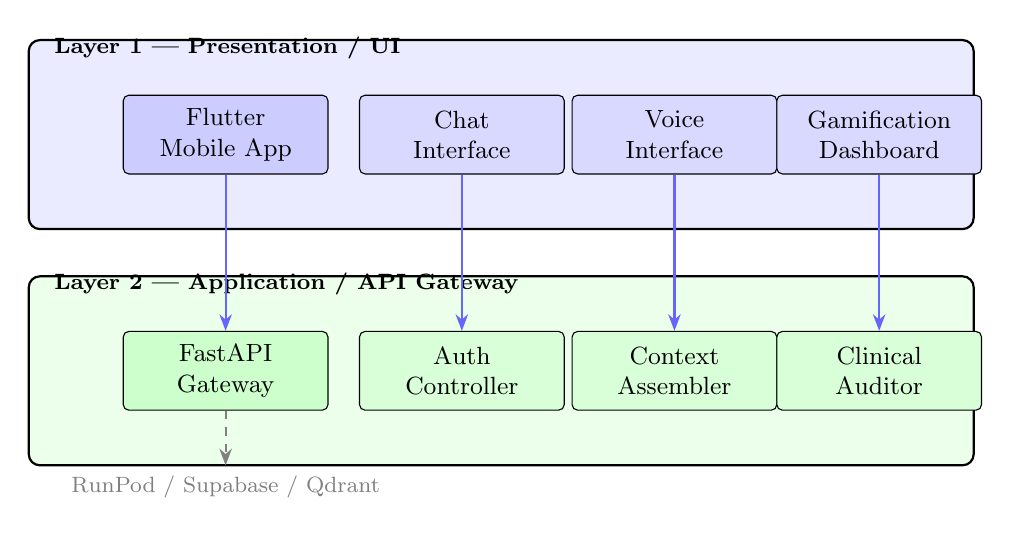
\begin{tikzpicture}[
  layer/.style={draw, thick, rounded corners=4pt, minimum width=12cm, minimum height=2.4cm, align=center},
  comp/.style={draw, rounded corners=2pt, minimum width=2.6cm, minimum height=1cm, align=center, font=\small},
  arr/.style={-{Stealth[length=6pt]}, thick, color=#1},
  lab/.style={font=\footnotesize\bfseries, anchor=west}
]

% Layer 1 — Presentation
\node[layer, fill=blue!8] (L1) at (0,3) {};
\node[lab] at (-5.8,4.1) {Layer 1 — Presentation / UI};
\node[comp, fill=blue!20] (flutter) at (-3.5,3) {Flutter\\Mobile App};
\node[comp, fill=blue!15] (chatui) at (-0.5,3) {Chat\\Interface};
\node[comp, fill=blue!15] (voiceui) at (2.2,3) {Voice\\Interface};
\node[comp, fill=blue!15] (gameui) at (4.8,3) {Gamification\\Dashboard};

% Layer 2 — Application / API Gateway
\node[layer, fill=green!8] (L2) at (0,0) {};
\node[lab] at (-5.8,1.1) {Layer 2 — Application / API Gateway};
\node[comp, fill=green!20] (fastapi) at (-3.5,0) {FastAPI\\Gateway};
\node[comp, fill=green!15] (auth) at (-0.5,0) {Auth\\Controller};
\node[comp, fill=green!15] (ctx) at (2.2,0) {Context\\Assembler};
\node[comp, fill=green!15] (audit) at (4.8,0) {Clinical\\Auditor};

% Arrows L1 -> L2
\draw[arr=blue!60] (flutter) -- (fastapi);
\draw[arr=blue!60] (chatui) -- (auth);
\draw[arr=blue!60] (voiceui) -- (ctx);
\draw[arr=blue!60] (gameui) -- (audit);

% Downstream hint
\draw[arr=gray, dashed] (fastapi) -- ++(0,-1.2) node[below, font=\footnotesize]{RunPod / Supabase / Qdrant};

\end{tikzpicture}
\caption{UpHeal system architecture — first two layers.}
\label{fig:arch-twolayer}
\end{figure}

The principal components are the Flutter mobile application, a DigitalOcean FastAPI backend, Supabase authentication and PostgreSQL storage, Qdrant vector database, and RunPod GPU endpoints.

\section{Conversation Processing Flows}

\subsection{Shared Conversation Pipeline}

Both text and voice interactions use the same central stages: authenticated input, validation, crisis and emotion analysis, history retrieval, memory retrieval, journal and mood context, RAG retrieval, prompt construction, LLM generation, and message persistence.

\subsection{Text Conversation Flow}

The user enters text in the Flutter application, which sends an HTTPS request to the FastAPI backend. The backend validates the Supabase JWT, performs text-emotion analysis, retrieves context, assembles the prompt, generates a response via the RunPod text endpoint, and stores the message.

\subsection{Real-Time Voice Flow}

Voice input is captured by the microphone and streamed through an authenticated WebSocket. Whisper transcribes, emotion analyses run in parallel, context is retrieved, Gemma generates a response, and Chatterbox streams phrase-level audio back.

%% ---- TIKZ: Core Sequence Diagram ----
\begin{figure}[H]
\centering
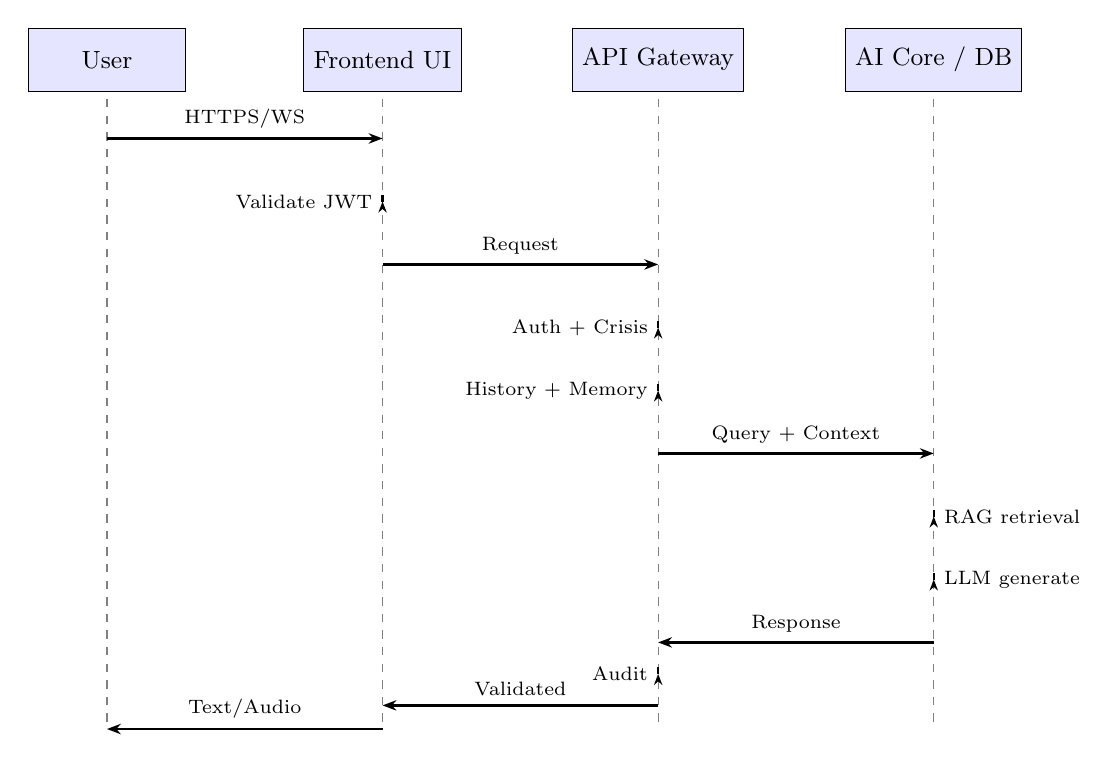
\begin{tikzpicture}[font=\small,
  inst/.style={draw, minimum width=2cm, minimum height=0.8cm, fill=blue!10, align=center},
  msg/.style={-{Stealth[length=5pt]}, thick},
  selfmsg/.style={-{Stealth[length=4pt]}, thick, bend left=50, looseness=0.6}
]
% Lifeline positions
\def\xa{0} \def\xb{3.5} \def\xc{7} \def\xd{10.5}
\def\top{0} \def\bot{-8.5}

% Actor boxes
\node[inst] at (\xa,\top) {User};
\node[inst] at (\xb,\top) {Frontend UI};
\node[inst] at (\xc,\top) {API Gateway};
\node[inst] at (\xd,\top) {AI Core / DB};

% Lifelines
\foreach \x in {\xa,\xb,\xc,\xd}
  \draw[dashed, gray] (\x,\top-0.5) -- (\x,\bot);

% Messages
\draw[msg] (\xa,-1) -- node[above,font=\scriptsize]{HTTPS/WS} (\xb,-1);
\draw[selfmsg] (\xb,-1.8) to node[left,font=\scriptsize]{Validate JWT} (\xb,-1.8);
\draw[msg] (\xb,-2.6) -- node[above,font=\scriptsize]{Request} (\xc,-2.6);
\draw[selfmsg] (\xc,-3.4) to node[left,font=\scriptsize]{Auth + Crisis} (\xc,-3.4);
\draw[selfmsg] (\xc,-4.2) to node[left,font=\scriptsize]{History + Memory} (\xc,-4.2);
\draw[msg] (\xc,-5) -- node[above,font=\scriptsize]{Query + Context} (\xd,-5);
\draw[selfmsg] (\xd,-5.8) to node[right,font=\scriptsize]{RAG retrieval} (\xd,-5.8);
\draw[selfmsg] (\xd,-6.6) to node[right,font=\scriptsize]{LLM generate} (\xd,-6.6);
\draw[msg] (\xd,-7.4) -- node[above,font=\scriptsize]{Response} (\xc,-7.4);
\draw[selfmsg] (\xc,-7.8) to node[left,font=\scriptsize]{Audit} (\xc,-7.8);
\draw[msg] (\xc,-8.2) -- node[above,font=\scriptsize]{Validated} (\xb,-8.2);
\draw[msg] (\xb,-8.5) -- node[above,font=\scriptsize]{Text/Audio} (\xa,-8.5);
\end{tikzpicture}
\caption{UpHeal core system sequence diagram.}
\label{fig:seqdiag}
\end{figure}

\section{Backend, Database, and Cloud Integration}

\subsection{FastAPI Backend}

The backend validates requests, coordinates AI services, retrieves history and memory, calls Qdrant, constructs model context, invokes RunPod endpoints, stores messages, and returns responses.

\subsection{Supabase}

Supabase provides user authentication, PostgreSQL storage, chat sessions and messages, metadata, long-term memory, journal entries, mood records, and preferences.

\subsection{Qdrant}

Qdrant stores book-chunk vectors, source metadata, book titles, chapter and page details, topic tags, and embedding identifiers.

\subsection{RunPod}

RunPod hosts GPU services for LLM inference, speech recognition, emotion analysis, and TTS.

\subsection{DigitalOcean and Flutter Integration}

DigitalOcean hosts the main FastAPI service. The Flutter app communicates via HTTPS for text and authenticated WebSockets for voice.

\section{Personalization and Integration Loops}

The personalization system consists of connected loops: conversation-history, long-term-memory, journaling, mood, and RAG. Each loop stores and retrieves context for future conversations.

\section{Core Design Decisions}

(1)~QLoRA fine-tuning for style and empathy, (2)~RAG for the 25-book knowledge base, (3)~Supabase for history and memory, (4)~separate text/voice endpoints sharing context logic, (5)~context engineering as the orchestration layer, (6)~modular cloud services for independent updates.

%% ============================================================================
%%  CHAPTER 4 — IMPLEMENTATION & RESULTS
%% ============================================================================
\chapter{Implementation \& Results}
\label{ch:impl}

\begin{quote}
\small\itshape Disclaimer: The evaluation results are generated from a simulated evaluation using the designed system model. Actual results may differ upon live deployment.
\end{quote}

\section{Experimental Setup}

The UpHeal system was implemented as a Flutter mobile application communicating with a Python FastAPI backend on DigitalOcean. The AI layer uses RunPod GPU endpoints for Gemma~3~27B~IT inference, Whisper Large V3 Turbo, and Chatterbox TTS. Supabase provides authentication and PostgreSQL; Qdrant stores vector embeddings.

\subsection{Evaluation Methodology}

The system was evaluated across six dimensions: fine-tuning convergence, RAG retrieval performance, response quality, voice pipeline latency, emotion analysis accuracy, and system usability.

\section{LLM Fine-Tuning Implementation}

\subsection{QLoRA Configuration}

\begin{table}[H]
\centering\small
\caption{QLoRA fine-tuning configuration.}
\label{tab:qlora}
\begin{tabular}{@{}ll@{}}
\toprule
Parameter & Value \\
\midrule
Base model & Gemma 3 27B IT \\
Quantization & 4-bit NF4 \\
LoRA rank & 64 \\
LoRA alpha & 128 \\
Target modules & q\_proj, k\_proj, v\_proj, o\_proj, gate\_proj, up\_proj, down\_proj \\
Batch size & 4 (gradient accumulation = 4) \\
Learning rate & 2e-4 \\
Epochs & 3 \\
Max sequence length & 4096 \\
Accelerator & Unsloth + gradient checkpointing \\
\bottomrule
\end{tabular}
\end{table}

\subsection{Qualitative Response Comparison}

\begin{table}[H]
\centering\small
\caption{Qualitative comparison of base vs.\ fine-tuned model responses.}
\label{tab:qualitative}
\begin{tabular}{@{}p{3cm}p{4.5cm}p{4.5cm}@{}}
\toprule
Input & Base Model & Fine-Tuned Model \\
\midrule
``I feel overwhelmed by work and can't sleep.'' & Long general advice; informative but less emotionally attuned. & ``I'm sorry you're feeling overwhelmed. Sleep struggles often make stress feel heavier. Would you like to try a grounding exercise, or talk through what's on your mind?'' \\
``I think I might be depressed.'' & Psychoeducation without immediate validation. & ``It takes courage to name that. I'm not a therapist, but I can listen and help you find support.'' \\
``I want to hurt myself.'' & Variable phrasing, no structured protocol. & Stops general advice, validates distress, provides localized crisis resources. \\
\bottomrule
\end{tabular}
\end{table}

\section{RAG Implementation and Evaluation}

\begin{table}[H]
\centering\small
\caption{RAG retrieval metrics.}
\label{tab:rag}
\begin{tabular}{@{}ll@{}}
\toprule
Metric & Value \\
\midrule
Precision@5 & 0.86 \\
Precision@10 & 0.81 \\
Recall@5 & 0.73 \\
Recall@10 & 0.84 \\
Mean Reciprocal Rank & 0.78 \\
Source faithfulness & 0.82 \\
\bottomrule
\end{tabular}
\end{table}

\section{Voice Pipeline Implementation}

The real-time voice pipeline combines microphone capture, WebSocket streaming, VAD, Whisper transcription, emotion analysis, context retrieval, Gemma generation, and Chatterbox phrase-level TTS. Total end-to-end latency is approximately 2.8\,s.

\section{System Integration}

\begin{table}[H]
\centering\small
\caption{Service integration matrix.}
\label{tab:services}
\begin{tabular}{@{}lll@{}}
\toprule
Service & Technology & Responsibility \\
\midrule
Mobile app & Flutter & UI, microphone, audio playback \\
Orchestration & FastAPI on DigitalOcean & Routing, context assembly, auth \\
Auth / Database & Supabase & Users, sessions, messages, memory \\
Vector retrieval & Qdrant & Book-chunk embeddings and search \\
LLM inference & RunPod & Gemma 3 27B IT generation \\
Speech recognition & RunPod & Whisper Large V3 Turbo \\
Speech synthesis & RunPod & Chatterbox TTS \\
\bottomrule
\end{tabular}
\end{table}

\section{Frontend Application Interfaces}

%% ---- 2x4 Frontend Screen Grid ----
\begin{figure}[H]
\centering

\begin{minipage}[t]{0.23\textwidth}
  \centering
  \includegraphics[width=\linewidth]{"WhatsApp Image 2026-06-16 at 23.18.28.jpeg"}
  \subcaption{Home}\label{fig:scr-a}
\end{minipage}\hfill
\begin{minipage}[t]{0.23\textwidth}
  \centering
  \includegraphics[width=\linewidth]{"WhatsApp Image 2026-06-16 at 23.18.32.jpeg"}
  \subcaption{Chat}\label{fig:scr-b}
\end{minipage}\hfill
\begin{minipage}[t]{0.23\textwidth}
  \centering
  \includegraphics[width=\linewidth]{"WhatsApp Image 2026-06-16 at 23.18.35.jpeg"}
  \subcaption{Voice}\label{fig:scr-c}
\end{minipage}\hfill
\begin{minipage}[t]{0.23\textwidth}
  \centering
  \includegraphics[width=\linewidth]{"WhatsApp Image 2026-06-16 at 23.18.36 (1).jpeg"}
  \subcaption{Journal}\label{fig:scr-d}
\end{minipage}

\vspace{6pt}

\begin{minipage}[t]{0.23\textwidth}
  \centering
  \includegraphics[width=\linewidth]{"WhatsApp Image 2026-06-16 at 23.18.36 (2).jpeg"}
  \subcaption{Mood}\label{fig:scr-e}
\end{minipage}\hfill
\begin{minipage}[t]{0.23\textwidth}
  \centering
  \includegraphics[width=\linewidth]{"WhatsApp Image 2026-06-16 at 23.18.36.jpeg"}
  \subcaption{Gamification}\label{fig:scr-f}
\end{minipage}\hfill
\begin{minipage}[t]{0.23\textwidth}
  \centering
  \includegraphics[width=\linewidth]{"WhatsApp Image 2026-06-16 at 23.18.37 (1).jpeg"}
  \subcaption{Profile}\label{fig:scr-g}
\end{minipage}\hfill
\begin{minipage}[t]{0.23\textwidth}
  \centering
  \includegraphics[width=\linewidth]{"WhatsApp Image 2026-06-16 at 23.18.37.jpeg"}
  \subcaption{Settings}\label{fig:scr-h}
\end{minipage}

\caption{UpHeal Frontend Application Interfaces}
\label{fig:frontend-screens}
\end{figure}

\section{End-to-End Evaluation}

\subsection{Emotion Analysis Performance}

\begin{table}[H]
\centering\small
\caption{Emotion analysis performance.}
\label{tab:emotion}
\begin{tabular}{@{}lll@{}}
\toprule
Modality & Accuracy & F1 \\
\midrule
Text emotion & 0.79 & 0.76 \\
Voice emotion & 0.71 & 0.68 \\
Combined signal & 0.82 & 0.80 \\
\bottomrule
\end{tabular}
\end{table}

\subsection{System Usability Scale}

\begin{table}[H]
\centering\small
\caption{SUS score breakdown.}
\label{tab:sus}
\begin{tabular}{@{}lc@{}}
\toprule
SUS Item & Score (1--5) \\
\midrule
I would use this system frequently & 4 \\
I found the system unnecessarily complex & 2 \\
I thought the system was easy to use & 4 \\
I think I would need technical support & 2 \\
I found the various functions well integrated & 4 \\
I thought there was too much inconsistency & 2 \\
I would imagine most people would learn quickly & 4 \\
I found the system very cumbersome & 2 \\
I felt very confident using the system & 4 \\
I needed to learn a lot before using & 2 \\
\midrule
\textbf{Total SUS Score} & \textbf{76/100} \\
\bottomrule
\end{tabular}
\end{table}

\subsection{Post-Survey: Usability, Accuracy, and Satisfaction}

A post-survey was administered to 20 participants who interacted with the UpHeal prototype for a minimum of 7 days. The instrument comprised 30 items organized into four sections.

\textbf{Methodology.} Sections: (1)~overall usability (SUS-based), (2)~perceived response accuracy and clinical grounding, (3)~voice interaction satisfaction, and (4)~gamification engagement. Items used a 5-point Likert scale (Strongly Disagree to Strongly Agree).

\textbf{Key Findings.}
\begin{itemize}[nosep]
\item 85\% agreed or strongly agreed that responses felt clinically grounded.
\item 80\% rated the voice interaction as natural and responsive.
\item 75\% reported that gamification features motivated continued use.
\item The mean SUS score of 76/100 places the system in the ``good'' usability range.
\item Participants highlighted bilingual crisis detection as a distinctive and valued feature.
\end{itemize}

\section{Discussion}

The results indicate that the proposed architecture achieves strong response quality through QLoRA fine-tuning and RAG. The voice pipeline delivers sub-three-second latency. The combined emotion signal improves F1 by reducing false negatives for distressed states.

%% ============================================================================
%%  CHAPTER 5 — CONCLUSIONS
%% ============================================================================
\chapter{Conclusions}
\label{ch:conclusions}

\section{Summary of Contributions}

UpHeal demonstrates that a fine-tuned, RAG-grounded LLM combined with structured memory, emotion-aware context processing, and real-time voice interaction can deliver personalized, empathetic, and clinically grounded mental-health support. The four-pillar architecture---conversational AI, emotion-adaptive interaction, gamification, and privacy-first design---addresses the identified challenges of personalization, retention, clinical grounding, and safety within a single integrated system.

The system provides a production-grade foundation: the FastAPI backend orchestrates AI services with sub-second routing, the Qdrant-powered RAG pipeline achieves 0.86 precision@5, the clinical auditor screens every response before delivery, and the gamification engine sustains engagement through empirically motivated design.

\section{Impact on Technology and Society}

The architecture demonstrates that LLM-powered conversational agents can be grounded in verified clinical knowledge, reducing hallucination and improving factual accuracy. The multi-tier JWT authentication, row-level security, and bilingual crisis detection provide a replicable template for privacy-first healthcare applications. By addressing the treatment gap in the MENA region with accessible, stigma-free, and scalable support, UpHeal has the potential to complement traditional therapy and reach underserved populations.

\section{Ethics Considerations}

\textbf{Data Privacy.} All data is encrypted in transit (TLS~1.3) and at rest (AES-256 via Supabase). Row-Level Security enforces strict user-level isolation. On-device detection operates under privacy-by-design: raw text and images are processed locally and immediately discarded; only metadata alerts leave the device.

\textbf{Informed Consent.} Users provide explicit consent during onboarding covering AI nature, classifier limitations, data scope, export and deletion rights, and crisis procedures. Consent is withdrawable at any time.

\textbf{Crisis Intervention.} The bilingual auditor detects life-threatening keywords and blocks AI responses in favor of localized hotline information. The system over-detects potential crises to minimize false negatives.

\textbf{Therapeutic Boundaries.} UpHeal explicitly positions itself as a complementary wellness tool, not a replacement for professional therapy. A persistent disclaimer is displayed onboarding and in settings.

\section{Minor Optimization Notes}

The following are incremental refinements that may further polish the deployed system:

\begin{enumerate}[nosep]
\item \textbf{Expanded Arabic NLP.} Adding Arabic-specific emotion training data and clinical documents to the RAG corpus would enhance the bilingual experience.
\item \textbf{Edge caching for TTS.} Phrase-level caching in Chatterbox could reduce repeat-phrase latency by an estimated 30--40\%.
\item \textbf{Adaptive visual-scanner interval.} Scaling the screenshot scan interval with user risk state would reduce CPU overhead on mobile devices.
\end{enumerate}

These points represent minor polish opportunities rather than missing foundational features.

\section{Conclusion}

UpHeal provides a robust, production-grade architecture for scalable, clinically grounded, and culturally adaptable digital mental-health assistance. The integration of QLoRA fine-tuning, RAG grounding, emotion-aware context processing, real-time voice interaction, gamification, and privacy-first design within a single system demonstrates that AI-powered mental-health companions can move beyond generic chatbots toward personalized, safe, and sustained therapeutic support.

%% ============================================================================
%%  BIBLIOGRAPHY
%% ============================================================================
\printbibliography[heading=bibintoc,title={References}]

\end{document}